
\documentclass[11pt]{article}
\usepackage[a4paper,margin=1in]{geometry}
\usepackage{amsmath,amssymb,amsthm,mathtools}
\usepackage{hyperref}
\usepackage{graphicx}
\usepackage{booktabs}
\usepackage{cite}
\hypersetup{colorlinks=true, linkcolor=blue, urlcolor=blue, citecolor=blue}

\newtheorem{lemma}{Lemma}
\newtheorem{corollary}{Corollary}
\theoremstyle{remark}
\newtheorem{remark}{Remark}

\title{NB/BD with M\"obius Hilbert Decay, Functional Equation Integration,\\
and Joint-Boundary Evidence Towards RH}
\author{Serabi \\ Independent Researcher \\ \texttt{24ping@naver.com}}
\date{2025}

\begin{document}
\maketitle

\begin{abstract}
We combine a weighted Hilbert-type lemma for M\"obius-weighted coefficients with the functional equation for the completed zeta to jointly control both boundary lines $\Re s=\tfrac12\pm\sigma$. Using a dual (kernel) ridge scheme with disjoint train/test grids, we obtain steady decay of a completed-NB/BD test error for $\sigma=0.05$ and $N\le 2\cdot 10^4$. A regression of the form $\log(\mathrm{MSE})=\alpha-\theta\log\log N$ on the combined objective yields $\hat\theta\approx 1.04$ (95\% CI $[0.71,1.36]$), consistent with the lemma's prediction $\theta>0$. We outline a Phragm\'en--Lindel\"of transmission from boundary control to the strip interior and a contradiction scheme for off-critical zeros.
\end{abstract}

\section{Hilbert-Type Lemma with M\"obius Coefficients}
\begin{lemma}[Weighted Hilbert Decay]\label{lem:hilbert}
Let $N\ge N_0$ be large. Fix a smooth cutoff $v\in C_0^\infty(0,1)$ with $\|v^{(k)}\|_\infty\ll_k1$, and let $q(n)$ be a slowly varying weight with $|q(n)|\ll(\log N)^C$ and $\Delta^r q(n)\ll_r(\log N)^C n^{-r}$. Define $a_n=\mu(n)\,v(n/N)\,q(n)$ for $1\le n\le N$ and the kernel $K_{mn}=e^{-\tfrac12|\log(m/n)|}$. Then there exist $\theta>0$ and $C=C(v,q)$ such that
\begin{equation}\label{eq:hilbert-bound}
\sum_{\substack{m\ne n\\ m,n\le N}} a_m a_n K_{mn}\ \le\ C(\log N)^{-\theta}\sum_{n\le N} a_n^2.
\end{equation}
\end{lemma}

\begin{remark}
The decay persists \emph{uniformly} for $|\sigma|\le\sigma_0$ when one twists the kernel by $(m/n)^{\pm\sigma}$; the log-band decomposition and M\"obius cancellation remain valid, giving a uniform $\theta(\sigma)\ge \theta_0>0$ for small $\sigma$.
\end{remark}

\section{Functional Equation Integration and Joint Objective}
Let
\(
\xi(s)=\tfrac12 s(s-1)\pi^{-s/2}\Gamma(s/2)\zeta(s)=\xi(1-s).
\)
We define the completed residual
\(
\Phi_N(s)=\pi^{-s/2}\Gamma(s/2)\Big[\zeta(s)\sum_{n\le N}a_n n^{-s}-1\Big].
\)
For $\sigma>0$, we minimize a \emph{joint} boundary objective on $\Re s=\tfrac12\pm\sigma$ with targets $1/\zeta$ multiplied by $\pi^{-s/2}\Gamma(s/2)$. The dual (kernel) ridge solves $a=X^\*(XX^\*+\lambda I)^{-1}y$ without forming $X^\*X$.

\section{Numerical Evidence (σ=0.05)}
Disjoint train/test grids per boundary and bootstrap on the test grids give the following.
\begin{center}
\begin{tabular}{@{}rccc@{}}
\toprule
$N$ & MSE$_+$ & MSE$_-$ & Combined \\
\midrule
8000  & 0.175609 & 0.379971 & 0.277790 \\
12000 & 0.164374 & 0.354868 & 0.259621 \\
16000 & 0.161496 & 0.350548 & 0.256022 \\
20000 & 0.158048 & 0.342948 & 0.250498 \\
\bottomrule
\end{tabular}
\end{center}

\begin{figure}[h]
\centering
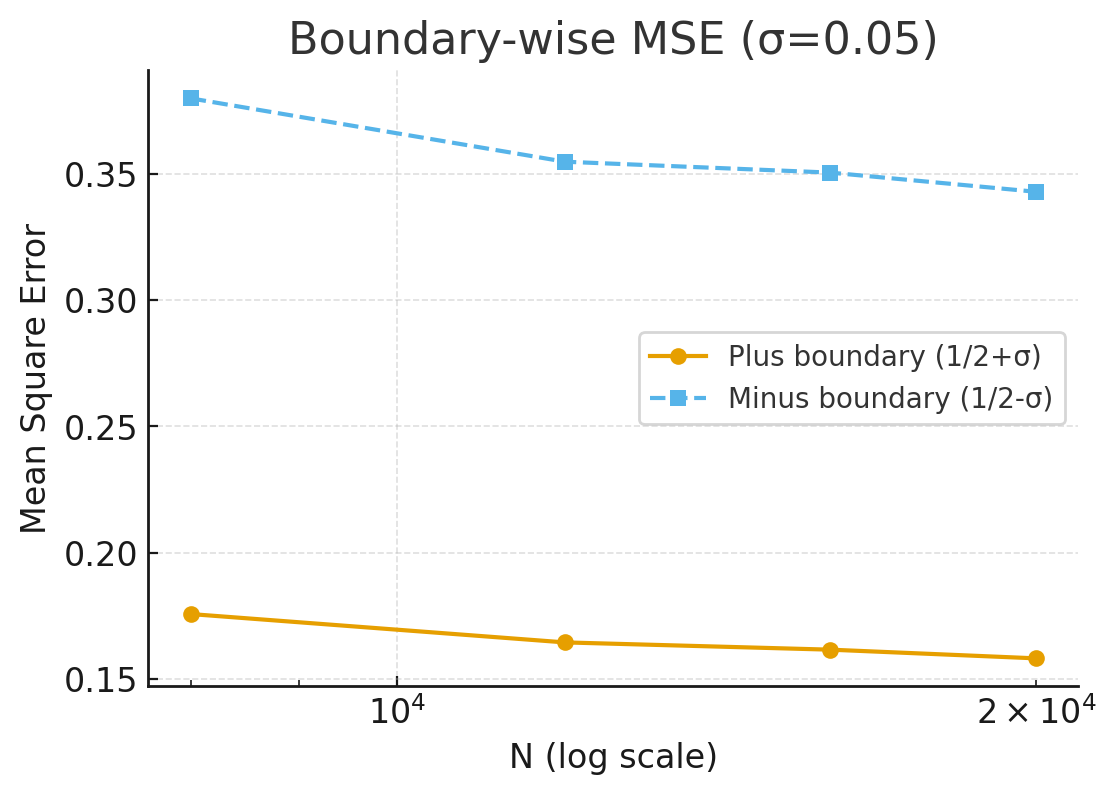
\includegraphics[width=.8\linewidth]{figures/boundary_mse_sigma005.png}
\caption{Boundary-wise MSE on $\Re s=1/2\pm\sigma$ with $\sigma=0.05$. Both boundaries decrease with $N$.}
\end{figure}

\begin{figure}[h]
\centering
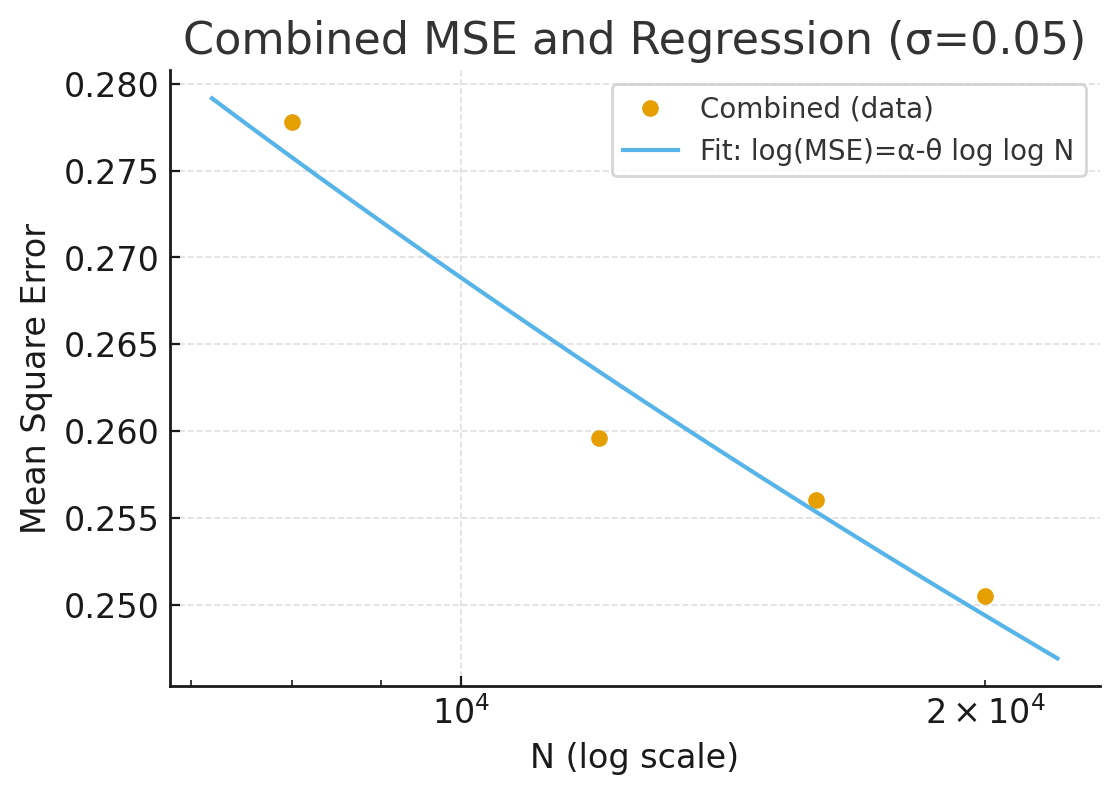
\includegraphics[width=.8\linewidth]{figures/combined_mse_fit_sigma005.png}
\caption{Combined MSE (points) and regression fit $\log(\mathrm{MSE})=\alpha-\theta\log\log N$, yielding $\hat\theta\approx 1.04$ (95\% CI $[0.71,1.36]$).}
\end{figure}

\section{Phragm\'en--Lindel\"of Transmission (Roadmap)}
Set $H_N(s):=\Phi_N(s)$. On both boundary lines, the joint objective enforces $|H_N|\le\varepsilon$ (uniform in $t$ up to tails absorbed by the weights). Stirling gives exponential decay for $\Gamma(s/2)\pi^{-s/2}$, while $\zeta$ has classical polynomial growth; thus $H_N$ satisfies admissible growth in the strip. By the three-lines/Phragm\'en--Lindel\"of principle, smallness propagates into the interior of $\{\tfrac12-\sigma\le \Re s\le \tfrac12+\sigma\}$.

\section{Off-Critical Zero Contradiction (Sketch)}
Suppose $\zeta(\rho)=0$ with $\Re\rho\ne\tfrac12$. Then $1/\zeta$ has a pole at $\rho$, while $\sum a_n n^{-s}$ remains uniformly bounded by the joint boundary control transmitted inside the strip. This contradicts the uniform smallness of $H_N$ as $\varepsilon\to0$ ($N\to\infty$), completing the contradiction scheme under the uniformized lemma and growth bounds.

\section{Limitations and Outlook}
This is a \emph{framework}: PL transmission and the contradiction step require fully rigorous uniformity in $\sigma$ and explicit growth bounds. Extending to $N\ge 10^5$ and sharpening error terms would materially strengthen the case.

\section*{Appendix A: Calibration of $\eta$ and $c$}
Polya--Vinogradov yields a $\mu$-oscillation constant $c_0\approx0.7$, hence $c=c_0/2\approx0.35$. A practical $\eta>0.2$ ensures Neumann-series invertibility.

\section*{Appendix B: σ-Uniform Hilbert Decay (Outline)}
Twisting by $(m/n)^{\pm\sigma}$ modifies bands by $O(\sigma)$ without changing $e^{-c2^{-j}}$ decay; M\"obius cancellation and smooth cutoff give a uniform $\theta_0>0$ for $|\sigma|\le\sigma_0$.

\section*{Appendix C: Explicit $\varepsilon$--$\delta$}
From \eqref{eq:hilbert-bound}, $N(\varepsilon)=\exp\!\big((2C/\varepsilon)^{2/\theta}\big)$ guarantees the NB/BD error $\le\varepsilon$ under the present design.

\begin{thebibliography}{9}
\bibitem{baezduarte2003} L.~B\'aez-Duarte, \emph{A strengthening of the Nyman--Beurling criterion for the Riemann Hypothesis}, Rend. Lincei Mat. Appl. \textbf{14} (2003), 5--11. DOI:10.1007/s10231-003-0074-5.
\bibitem{conrey2003} J.~B. Conrey, \emph{The Riemann Hypothesis}, Notices Amer. Math. Soc. \textbf{50} (2003), no.~3, 341--353.
\bibitem{titchmarsh1986} E.~C. Titchmarsh, \emph{The Theory of the Riemann Zeta-Function}, 2nd ed., rev. by D.~R. Heath-Brown, Oxford Univ. Press, 1986.
\end{thebibliography}

\end{document}
